\iffalse
\chapter{2020}
\section{ae}
\author{AI24BTECH11023 - Tarun Reddy Pakala}
\fi
\item The positive high angle-of-attack condition is obtained in a steady pull-out maneuver at the largest permissible angle-of-attack of the wing. Under this condition, at which of the following regions of the wing does the maximum tension occur?
%input for figure 1
\begin{center}  % Centering environment
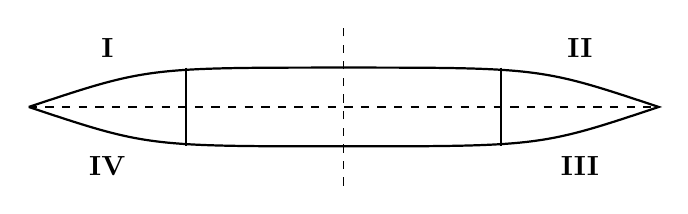
\begin{tikzpicture}
  % Draw the main airfoil shape
  \draw[thick] 
    (0,0) 
    .. controls (1.5,0.5) .. (4,0.5) % Upper curve
    .. controls (6.5,0.5) .. (8,0)   % Upper curve continuation
    .. controls (6.5,-0.5) .. (4,-0.5) % Lower curve
    .. controls (1.5,-0.5) .. (0,0);  % Lower curve continuation

  % Vertical lines for reference points
  \draw[thick] (2,0.5) -- (2,-0.5);
  \draw[thick] (6,0.5) -- (6,-0.5);

  % Centerline
  \draw[dashed] (0,0) -- (8,0);

  % Axis line at midpoint
  \draw[dashed] (4,-1) -- (4,1);

  % Labels for sections
  \node at (1,0.75) {\textbf{I}};
  \node at (7,0.75) {\textbf{II}};
  \node at (7,-0.75) {\textbf{III}};
  \node at (1,-0.75) {\textbf{IV}};

\end{tikzpicture}
\end{center}

\begin{enumerate}
    \item $I$
    \item $II$
    \item $III$
    \item $IV$
\end{enumerate}
\item The natural frequency of the first mode of a rectangular cross section cantilever aluminum beam is $\omega \frac{rad}{s}$. If the material and cross-section remain the same, but the length of the beam is doubled, the first mode frequency will become
\begin{enumerate}
    \item $\frac{\omega}{4}\frac{rad}{s}$
    \item $4\omega \frac{rad}{s}$
    \item $\frac{\omega}{16} \frac{rad}{s}$
    \item $16\omega \frac{rad}{s}$
\end{enumerate}
\item Given $A=\begin{pmatrix}
    \sin \theta & \tan \theta \\
    0 & \cos \theta \\
\end{pmatrix}$, the sum of squares of eigenvalues of $A$ is
\begin{enumerate}
    \item $\tan^2\theta$
    \item $1$
    \item $\sin^2\theta$
    \item $\cos^2\theta$
\end{enumerate}
\item Burnout velocity of a space vehicle in a circular orbit at angle $5$ degrees above the local horizon around earth is $13.5\;\frac{km}{s}$. Tangential velocity of the space vehicle in the orbit is \underline{\hspace{2cm}} $\frac{km}{s}$ \brak{round\;off\;to\;two\;decimal\;places}.
\item Velocity of an airplane in the body fixed axes is given as $\sbrak{100\;-10\;20} \frac{m}{s}$. The sideslip angle is \underline{\hspace{2cm}} degrees \brak{round\;off \;to \;two\; decimal\; places}.
\item The similarity solution for the diffusion equation,$\frac{\partial u}{\partial t}=\alpha \frac{\partial^2u}{\partial x^2}$ is $u\brak{x,\;t}=u\brak{\eta}$, where similarity variable, $\eta=\frac{x}{\sqrt{\alpha t}}$. If $u\brak{x\;0}=e^{-x^2}$, the ratio $\frac{u\brak{0,\;1}}{u\brak{0\;4}}=$ \underline{\hspace{2cm}} \brak{round \; off \; to\; one \; decimal\;place }.
\item Air enters the rotor of an axial compressor stage with no pre-whirl \brak{C_\theta=0} and exits the rotor with whirl velocity, $C_\theta=150\frac{m}{s}$. The velocity of rotor vanes, $U$ is $200 \frac{m}{s}$. Assume $C_P=100\frac{J}{kg\;K}$, the stagnation temperature rise across the rotor is \underline{\hspace{2cm}} $K$ \brak{round\;off\;to\;one\;decimal\;place}.
\item A thin walled beam of constant thickness shown in the figure is subjected to a torque of $3.2\;kNm$. If the shear modulus is $25 GPa$, the angle of twist per unit length is \underline{\hspace{2cm}} $\frac{rad}{m}$ \brak{round\;off\;to\;three\;decimals}.
%input for figure 2
\begin{figure}[H]
\centering
\resizebox{3cm}{3cm}{%
\begin{circuitikz}
\tikzstyle{every node}=[font=\small]
\draw  (2.5,11.75) rectangle (12.5,8.5);
\node [font=\small] at (7,12.25) {$400 \;mm$};
\node [font=\small] at (11.25,10.25) {$2\; mm$};
\node [font=\small] at (1.75,10) {$100 \;mm$};
\draw [->, >=Stealth] (1.75,9.75) -- (1.75,8.5);
\draw [->, >=Stealth] (1.75,10.25) -- (1.75,11.75);
\draw [->, >=Stealth] (6.25,12.25) -- (2.5,12.25);
\draw [->, >=Stealth] (7.5,12.25) -- (12.5,12.25);
\draw [->, >=Stealth] (11.75,10.25) -- (12.5,10.25);
\draw [->, >=Stealth] (13.25,10.25) -- (12.5,10.25);
\end{circuitikz}
}%

\label{fig:my_label}
\end{figure}

\item An airplane of mass $5000\;kg$ is flying at a constant speed of $360\;\frac{km}{h}$ at the bottom of a vertical circle with a radius of $400\;m$, as shown in the figure. Assuming that the acceleration due to gravity is $9.8\;\frac{m}{s^2}$, the load factor experienced at the center of gravity of the airplane is \underline{\hspace{2cm}} \brak{round\;off\;to\;two\;decimal\;places}. 
%input for figure 3
\begin{center}
\begin{tikzpicture}
  % Draw the curved path
  \draw[dashed] (-6,0) .. controls (0, -2) .. (6,0);

  % Draw the airplane
  \draw[thick] (0,-2) 
    -- ++(1,0) arc[start angle=0, end angle=180, radius=1cm] -- cycle; % Airplane wings
  \draw (0,-2) ellipse (1.5cm and 0.3cm); % Elliptical fuselage

  % Label
  \node at (0,-3) {Airplane};

\end{tikzpicture}
\end{center}

\item The equation $x\frac{dx}{dy}+y=c$, where $c$ is a constant, represents a family of
\begin{enumerate}
    \item exponential curves 
    \item parabolas 
    \item circles
    \item hyperbolas
\end{enumerate}
\item A wedge shaped airfoil is placed in a supersonic flow as shown in figure \brak{\text{not to scale}}. The corners of the wedge are at $x=\text{x}_A$, $x=\text{x}_B$,\;$x=\text{x}_C$, respectively.\\
%input for figure 4
\begin{figure}[H]
\centering
\resizebox{3cm}{3cm}{%
\begin{circuitikz}
\tikzstyle{every node}=[font=\small]
\draw [->, >=Stealth] (3.5,10.75) -- (3.5,13.75);
\draw [->, >=Stealth] (3.5,10.75) -- (10.75,10.75);
\draw [->, >=Stealth] (2.25,10.75) -- (3.25,10.75);
\draw [dashed] (4.5,13.25) -- (4.5,8.25);
\draw [dashed] (7.25,13.25) -- (7.25,8.25);
\draw [dashed] (10,13.25) -- (10,8.25);
\draw [dashed] (2,8.25) -- (10,8.25);
\draw [dashed] (2,13) -- (10,13);
\draw [short] (4.5,10.75) -- (7.25,11.75);
\draw [short] (7.25,11.75) -- (10,9.75);
\draw [short] (4.5,10.75) -- (10,9.75);
\node [font=\small] at (2.5,11) {$M>1$};
\node [font=\small] at (3.5,14) {$y$};
\node [font=\small] at (11,10.75) {$x$};
\node [font=\small] at (4.5,8) {$X_A$};
\node [font=\small] at (7.25,8) {$X_B$};
\node [font=\small] at (10,8) {$X_C$};
\node [font=\small] at (1.75,8.25) {$Y_{II}$};
\node [font=\small] at (1.75,13) {$Y_I$};
\node [font=\small] at (5.5,11) {$\alpha$};
\node [font=\small] at (6.5,10.5) {$\alpha$};
\node [font=\small] at (9,10) {$2\alpha$};
\end{circuitikz}
}%
\label{fig:my_label}
\end{figure}

Which one of the following represents the correct static pressure along $y=\text{Y}_I$ and $y=\text{Y}_{II}$?
\begin{enumerate}
    \item 
    %input for figure 5
    \begin{figure}[H]
\raggedright% Align the figure to the left
\resizebox{3cm}{3cm}{%
\begin{circuitikz}
\tikzstyle{every node}=[font=\small]
\draw [->, >=Stealth] (0.5,8) -- (0.5,12.5);
\draw [->, >=Stealth] (0.5,8) -- (6.5,8);
\draw [->, >=Stealth] (7,8) -- (13.25,8);
\draw [->, >=Stealth] (7,8) -- (7,12.5);
\draw [dashed] (1,12) -- (1,8.5);
\draw [dashed] (3,12) -- (3,8.75);
\draw [dashed] (5,12) -- (5,8.5);
\draw [short] (0.5,9.5) -- (1,9.5);
\draw [short] (1,9.5) -- (1,11.5);
\draw [short] (1,11.5) -- (3.5,11.5);
\draw [short] (3.5,11.5) -- (4.25,9.25);
\draw [short] (4.25,9.25) -- (5,9.25);
\draw [dashed] (7.5,12.25) -- (7.5,8.75);
\draw [dashed] (9.5,12.25) -- (9.5,8.75);
\draw [dashed] (12,12.25) -- (12,9);
\draw [short] (7,9.75) -- (7.5,9.75);
\draw [short] (7.5,11.75) -- (12,11.75);

\node [font=\small] at (8.5,12) {$Y_{II}$};
\node [font=\small] at (7.5,8.5) {$X_A$};
\node [font=\small] at (9.5,8.5) {$X_B$};
\node [font=\small] at (12,8.75) {$X_C$};
\node [font=\small] at (1,8.25) {$X_A$};
\node [font=\small] at (3,8.5) {$X_B$};
\node [font=\small] at (5,8.5) {$X_C$};
\node [font=\small] at (6.5,11.25) {P};
\node [font=\small] at (0.25,11.5) {P};
\node [font=\small] at (4,7.75) {$x$};
\node [font=\small] at (10.5,7.75) {$x$};
\node [font=\small] at (1.75,11.75) {$Y_I$};

\end{circuitikz}%
}
\end{figure}

    \item 
    %input for figure 6
    \begin{figure}[H]
\raggedright
\resizebox{3cm}{3cm}{%
\begin{circuitikz}
\tikzstyle{every node}=[font=\small]
\draw [->, >=Stealth] (0.5,8) -- (0.5,12.5);
\draw [->, >=Stealth] (0.5,8) -- (6.5,8);
\draw [->, >=Stealth] (7,8) -- (13.25,8);
\draw [->, >=Stealth] (7,8) -- (7,12.5);
\draw [dashed] (1,12) -- (1,8.5);
\draw [dashed] (3,12) -- (3,8.75);
\draw [dashed] (5,12) -- (5,8.5);
\draw [short] (0.5,9.5) -- (1,9.5);
\draw [short] (1,9.5) -- (1,11.5);
\draw [short] (1,11.5) -- (3.5,11.5);
\draw [short] (3.5,11.5) -- (4.25,9.25);
\draw [short] (4.25,9.25) -- (5,9.25);
\draw [dashed] (7.5,12.25) -- (7.5,8.75);
\draw [dashed] (9.5,12.25) -- (9.5,8.75);
\draw [dashed] (12,12.25) -- (12,9);
\draw [short] (7,9.75) -- (7.5,9.75);
\draw [short] (7.5,11.75) -- (12,11.75);
\node [font=\small] at (8.5,12) {$Y_{II}$};
\node [font=\small] at (7.5,8.5) {$X_A$};
\node [font=\small] at (9.5,8.5) {$X_B$};
\node [font=\small] at (12,8.75) {$X_C$};
\node [font=\small] at (1,8.25) {$X_A$};
\node [font=\small] at (3,8.5) {$X_B$};
\node [font=\small] at (5,8.5) {$X_C$};
\node [font=\small] at (6.5,11.25) {P};
\node [font=\small] at (0.25,11.5) {P};
\node [font=\small] at (4,7.75) {$x$};
\node [font=\small] at (10.5,7.75) {$x$};
\node [font=\small] at (1.75,11.75) {$Y_I$};
\draw [short] (7.5,9.75) -- (7.5,11.75);
\end{circuitikz}
}%
\end{figure}

    \item 
    %input for figure 7
    \begin{figure}[H]
\raggedright
\resizebox{3cm}{3cm}{%
\begin{circuitikz}
\tikzstyle{every node}=[font=\small]
\draw [->, >=Stealth] (0.5,8) -- (0.5,12.5);
\draw [->, >=Stealth] (0.5,8) -- (6.5,8);
\draw [->, >=Stealth] (7,8) -- (13.25,8);
\draw [->, >=Stealth] (7,8) -- (7,12.5);
\draw [dashed] (1,12) -- (1,8.5);
\draw [dashed] (3,12) -- (3,8.75);
\draw [dashed] (5,12) -- (5,8.5);
\draw [short] (0.5,9.5) -- (1,9.5);
\draw [short] (1,9.5) -- (1,11.5);
\draw [short] (1,11.5) -- (3.5,11.5);
\draw [dashed] (7.5,12.25) -- (7.5,8.75);
\draw [dashed] (9.5,12.25) -- (9.5,8.75);
\draw [dashed] (12,12.25) -- (12,9);
\node [font=\small] at (8.5,12) {$Y_{II}$};
\node [font=\small] at (7.5,8.5) {$X_A$};
\node [font=\small] at (9.5,8.5) {$X_B$};
\node [font=\small] at (12,8.75) {$X_C$};
\node [font=\small] at (1,8.25) {$X_A$};
\node [font=\small] at (3,8.5) {$X_B$};
\node [font=\small] at (5,8.5) {$X_C$};
\node [font=\small] at (6.5,11.25) {P};
\node [font=\small] at (0.25,11.5) {P};
\node [font=\small] at (4,7.75) {$x$};
\node [font=\small] at (10.5,7.75) {$x$};
\node [font=\small] at (1.75,11.75) {$Y_I$};
\draw [short] (7,9.5) -- (8,9.5);
\draw [short] (8,9.5) -- (8,11.75);
\draw [short] (8,11.75) -- (12,11.75);
\draw [short] (3.5,11.5) -- (3.5,9);
\draw [short] (3.5,9) -- (5,9);
\end{circuitikz}
}%

\label{fig:my_label}
\end{figure}

    \item 
    %input for figure 8
    \begin{figure}[H]
\raggedright
\resizebox{3cm}{3cm}{%
\begin{circuitikz}
\tikzstyle{every node}=[font=\small]
\draw [->, >=Stealth] (0.5,8) -- (0.5,12.5);
\draw [->, >=Stealth] (0.5,8) -- (6.5,8);
\draw [->, >=Stealth] (7,8) -- (13.25,8);
\draw [->, >=Stealth] (7,8) -- (7,12.5);
\draw [dashed] (1,12) -- (1,8.5);
\draw [dashed] (3,12) -- (3,8.75);
\draw [dashed] (5,12) -- (5,8.5);
\draw [short] (0.5,9.5) -- (1,9.5);
\draw [short] (1,9.5) -- (1,11.5);
\draw [short] (1,11.5) -- (3.5,11.5);
\draw [short] (3.5,11.5) -- (4.25,9.25);
\draw [short] (4.25,9.25) -- (5,9.25);
\draw [dashed] (7.5,12.25) -- (7.5,8.75);
\draw [dashed] (9.5,12.25) -- (9.5,8.75);
\draw [dashed] (12,12.25) -- (12,9);
\node [font=\small] at (8.5,12) {$Y_{II}$};
\node [font=\small] at (7.5,8.5) {$X_A$};
\node [font=\small] at (9.5,8.5) {$X_B$};
\node [font=\small] at (12,8.75) {$X_C$};
\node [font=\small] at (1,8.25) {$X_A$};
\node [font=\small] at (3,8.5) {$X_B$};
\node [font=\small] at (5,8.5) {$X_C$};
\node [font=\small] at (6.5,11.25) {P};
\node [font=\small] at (0.25,11.5) {P};
\node [font=\small] at (4,7.75) {$x$};
\node [font=\small] at (10.5,7.75) {$x$};
\node [font=\small] at (1.75,11.75) {$Y_I$};
\draw [short] (7,9.5) -- (8,9.5);
\draw [short] (8,9.5) -- (8,11.75);
\draw [short] (8,11.75) -- (12,11.75);
\end{circuitikz}
}%

\end{figure}

\end{enumerate}
\item The value of Poisson's ratio at which the shear modulus of an isotropic material is equal to the bulk modulus is
\begin{enumerate}
    \item $\frac{1}{2}$
    \item $\frac{1}{4}$
    \item $\frac{1}{6}$
    \item $\frac{1}{8}$
\end{enumerate}
\item A load P is applied to the free end of a stepped cantilever beam as shown in the figure. The Young's modulus of the material is $E$, and the moments of inertia of the two sections of length $2\;m$ and $1\;m$ are $I$ and $3I$, respectively. Ignoring transverse shear and stress concentration effects, the deflection at the point where the load is applied at the free end of the cantilever is  
%input for figure 9
\begin{figure}[H]
\centering
\resizebox{3cm}{3cm}{%
\begin{circuitikz}
\tikzstyle{every node}=[font=\large]
\draw [ line width=0.9pt ] (9,12) rectangle (12.5,10.25);
\draw [ line width=0.9pt ] (9,11.5) rectangle (4,10.75);
\draw [line width=2pt, ->, >=Stealth] (4,10.75) -- (4,9.75);
\draw [line width=0.5pt, dashed] (9,12) -- (11,12);
\draw [line width=0.5pt, dashed] (9,12) -- (9,13);
\draw [line width=1.1pt, short] (12.5,12.5) -- (12.5,9.75);
\node [font=\small] at (10.5,12.5) {$1\;m$};
\node [font=\small] at (6,12.5) {$2\;m$};
\node [font=\small] at (4.5,10) {$P=3\;N$};
\draw [line width=0.6pt, ->, >=Stealth] (6.25,12.5) -- (9,12.5);
\draw [line width=0.6pt, ->, >=Stealth] (10,12.5) -- (9,12.5);
\draw [line width=0.6pt, dashed] (4,11.5) -- (4,13);
\draw [line width=0.6pt, dashed] (12.5,12.5) -- (12.5,13);
\draw [line width=0.6pt, ->, >=Stealth] (5.75,12.5) -- (4,12.5);
\draw [line width=0.6pt, ->, >=Stealth] (10.75,12.5) -- (12.5,12.5);
\node [font=\large] at (10.75,11.25) {$3I$};
\node [font=\large] at (6.5,11.25) {$I$};
\end{circuitikz}
}%

\label{fig:my_label}
\end{figure}

\begin{enumerate}
    \item $\frac{23}{243EI}$
    \item $\frac{1}{3EI}$
    \item $\frac{43}{3EI}$
    \item $\frac{23}{3EI}$
\end{enumerate}


